\section{Testing}

This section covers property testing using QuickCheck, system testing using a 
built-in test suite and MySQL WorkBench for SQL query testing. EFA's 
implementation uses dependent types which express application-specific program 
invariants that are beyond the scope of existing type systems. The tests that 
are implemented make two assumptions, the first being any element reused from 
the Ampersand system is already correct, and the second being that if the 
properties of a function are correctly implemented, when used in combination 
with assumption one that the outcome is correct.

\subsection{Property Testing Using QuickCheck}
Not all functions can be tested using QuickCheck due to their complexity (e.g. 
eca2SQL). All of EFA's modules rely on a few base modules, and testing the 
properties of the functions implemented in the base modules, by extension, 
tests all functions that rely on these core modules. These tests can be checked 
using stack and running \verb|``quickCheck <function>''|. The data types are 
presumed correct as they produce the correct results and are accepted by the 
Ampersand system. Furthermore, proof of EFA's TypedSQL was provided in software 
implementation section \ref{subsec:modhierarchy}
\begin{center}
     \begin{adjustwidth}{-2cm}{}
    \begin{longtable}{ |m{1.8cm}|m{3.2cm}|m{9cm}| } 
        \hline
         Module & Function & Test Description \\ 
        \hline \hline
         Singletons & singKindWitness1 & For every pair of types 
        and their type representation, an isomorphism exists, where an 
        isomorphism is a morphism $f:\ a \rightarrow b$ and there exists a 
        morphism $g: b \rightarrow a$ with $fg$ = $1_b$ and $gf$ = $1_a$.
        \\  & & 
        \\  & & The 
        default implementation uses UnsafeCoerce and will only work if 
        everything is correctly defined.    
         
        \\\hline 
        Singletons & sing2val & sing2val takes a singleton and returns a value, 
        \\ &val2sing & while val2sing does the opposite, composing these two 
         functions together should return the same output as the given input. 
         \\  & &
         \\  & & $val2sing\ x (sing2val\ x) \equiv \ x$ 
         \\  & & $sing2val\ x (val2sing\ x) \equiv \ x$
         
         \\\hline
        Singletons& $\%==$ & Tests for equality by checking for transitivity, 
        symmetry and reflexivity.
        
        \\ & & Transitive relation: 
        \\ & &  
        $\forall\ a,\ b,\ c \in  X$ : ($aRb \wedge bRc$)$ \Rightarrow\ aRc$
        
        \\ & & Reflexive relation:
        \\ & & 
        $\forall a \in\ X $($aRa$)   
         
        \\ & & Symmetry relation:
        \\ & &
        $\forall a, b, \in X$ ($aRb \Rightarrow bRa$)
        \\ \hline
        Utils & prod2sing & prod2sing is the opposite of sing2prod using this \\
              & sing2prod  & logic composing the two functions should return 
              the same output irregardless of order. 
          \\  & &
          \\  & & $prod2sing\ x (sing2prod\ x) \equiv \ x$ 
          \\  & & $sing2prod\ x (prod2sing\ x) \equiv \ x$
          \\\hline
          & & \\
        Utils & prod2sing & prod2sing is the opposite of sing2prod using this \\
        & sing2prod  & logic composing the two functions should return 
        the same output irregardless of order. 
        \\  & &
        \\  & & $prod2sing\ x (sing2prod\ x) \equiv \ x$ 
        \\  & & $sing2prod\ x (prod2sing\ x) \equiv \ x$
        \\\hline
         & & \\
        Utils & prod2sing & prod2sing is the opposite of sing2prod using this \\
        & sing2prod  & logic composing the two functions should return 
        the same output irregardless of order. 
        \\  & &
        \\  & & $prod2sing\ x (sing2prod\ x) \equiv \ x$ 
        \\  & & $sing2prod\ x (prod2sing\ x) \equiv \ x$
        \\\hline
        & & \\
        Utils & foldrProd  &  These functions can be tested using conventional\\
              & foldlProd  & methods as they are analogous to the built-in\\
              & zipProd &  haskell functions.\\
              & mapProd & \\
        \\ \hline        
\end{longtable}
\end{adjustwidth}
\end{center}

\subsection{System Testing Using Test suite}
The test suite runs by using the cabal system and running 
\verb|``cabal configure --enable-tests''|; this test suite was built 
specifically for EFA and 
more details are provided in the 
\href{https://github.com/4ZP6Capstone2015/ampersand/blob/master/src/Database/Design/Ampersand/ECA2SQL/FreshName.lhs}{literate
 source code} located in EFA's github repository.

\subsection{Manual Execution of EFA's SQL Queries}

The queries produced by EFA were manually tested on a MySQL server; Ampersand 
relies on a MySQL database which can be installed as a part of xampp along with 
apache or simply on its own from the 
\href{https://dev.mysql.com/downloads/mysql/}{MySQL website}. A simple guide is 
available in the appendix \ref{appen:SQL}, on how to install a MySQL Database 
through xampp and MySQL; instructions are provided on how to use xampp's MySQL 
server with MySQL WorkBench. Furthermore, 
\href{https://dev.mysql.com/downloads/workbench/}{WorkBench} can be found on 
MySQL's official website.

Xampp must be running Apache and MySQL for WorkBench to be able to connect to 
the database server. 
\begin{figure}[!h]
    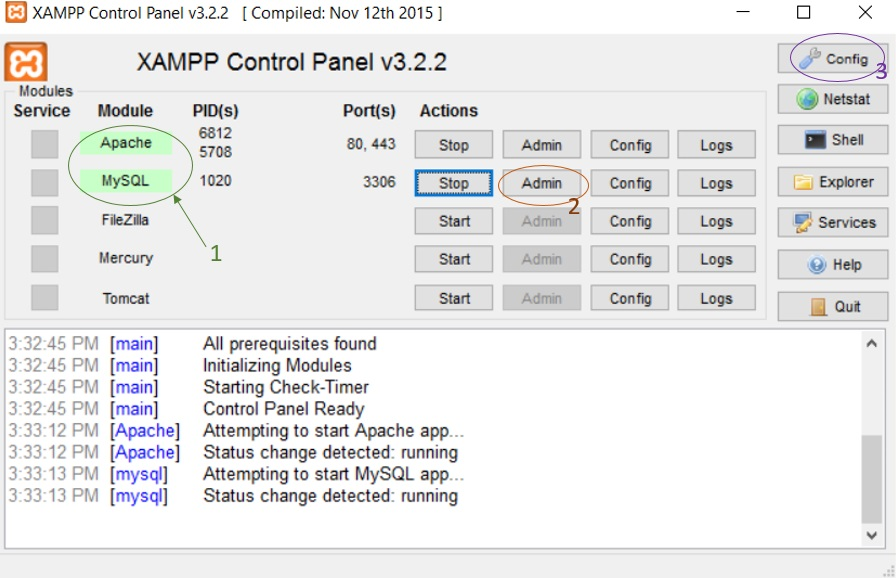
\includegraphics[width=\textwidth]{images/xampp}
    \caption{\footnotesize{1. Shows that both and Apache and MySQL must be 
    running at the same time. 2. The Admin button for mySQL opens phpAdmin 
    which is an graphical interface for accessing the databases in an MySQL 
    server. 3. Configuration button $\rightarrow$ services and ports 
    $\rightarrow$ [MySQL] tab, check that the port is identical to the 
    connected established for WorkBench. The standard is port 3306 }}
\end{figure}

Queries can be executed manually using WorkBench, to follow instructions on how 
to set up a connection for WorkBench, please refer to appendix 
\ref{appen:WorkBench}. Once Work Bench is running properly, it will very 
similar to screen shot provided.
\begin{figure}[!h]
    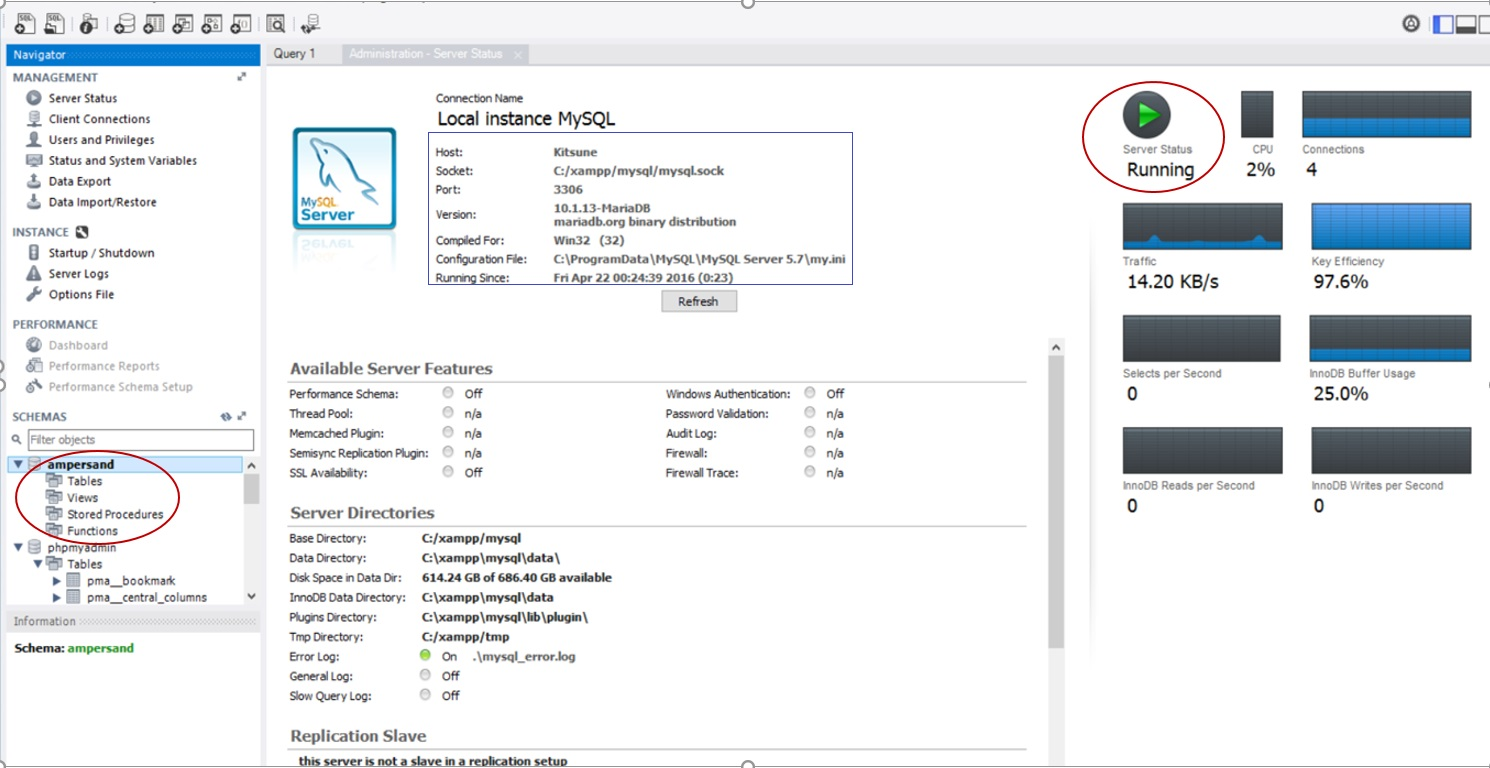
\includegraphics[width=\textwidth]{images/WorkBench}
    \caption{\footnotesize{The right-hand side shows the status of the server, 
    and on the lower left-hand side under 'SCHEMAS', all the databases in 
    current server is listed. Ampersand requires a local database and a 
    password, both of which are 'ampersand'. The blue box in the top middle 
    area provides information concerning the host. }}
\end{figure}

Queries are executed by going to [File] $\rightarrow$ [New Query Tab], a new 
tab will open and one can manually type queries. The execution of these queries 
can be specified to the highlighted portion or everything. The pretty-printer 
can be used to print the translated ECA rules and the associated queries.
